\documentclass[10pt]{report}
\usepackage[utf8]{inputenc}
\usepackage[greek]{babel}
\usepackage{tikz} 
\usepackage{listings}
\newcommand{\en}{\selectlanguage{english}}
\newcommand{\gr}{\selectlanguage{greek}}
\usepackage{fancyhdr}
\pagestyle{plain}
\fancyhf{}
\fancyhead[R]{\leftmark \gr ΛΕΚΚΑΣ ΓΕΩΡΓΙΟΣ ΑΜ:1067430}
\fancyhead[LO]{\rightmark }
\fancypagestyle{plain}{}
\usepackage{graphicx}
\usepackage{amsthm}
\usepackage{amssymb}
\usepackage{geometry}
\geometry{
	a4paper,
	total={170mm,257mm},
	left=20mm,
	top=20mm,
}
\usepackage{subfig}

\title{\textbf{2o  {\en PROJECT} ΑΠΟΚΕΝΤΡΩΜΕΝΟΣ ΥΠΟΛΟΓΙΣΜΟΣ \& ΜΟΝΤΕΛΟΠΟΙΗΣΗ}}
\author{\gr ΛΕΚΚΑΣ ΓΕΩΡΓΙΟΣ ΑΜ:1067430  Έτος 5ο\newline}
\date{}
\cfoot{\thepage}
\begin{document}
	\maketitle	
	\thispagestyle{fancy}
	\tableofcontents
	\pagestyle{plain}
	\begin{itemize}
		\item[A.] \gr Θεωρητική Άσκηση 1 
		\item[Β.] \gr Θεωρητική Άσκηση 2
		\item[Γ.] \gr Προγραμματιστική Άσκηση 1
		\item[Δ.] \gr Προγραμματιστική Άσκηση 2
		
	\end{itemize}
	\pagebreak
	\gr Η συγγραφή της αναφοράς πραγματοποιήθηκε σε {\en Latex} με τη βοήθεια του {\en TexStudio}.\\ \\ 
	\section*{\gr \textbf{Α.Θεωρητική Άσκηση 1}}
	
	\gr Το πρώτο βήμα που πρέπει να γίνει για να αποδείχθεί αν ένας αλγόριθμος είναι αυτοσταθεροποιητικός ή όχι είναι να περιορίσουμε τον δαίμονα,δηλαδή το "περιβάλλον", αυτόν που καθορίζει τις εισόδους.Οπότε για τη συγκεκριμένη απόδειξη θα χρησιμοποιήσουμε έναν {\en Locally Central Unfair Deamon}.{\en Locally Central } διότι επιλέγουμε να μην ενεργοποιούνται δυο διαδοχικοί κόμβοι στο ίδιο βήμα και {\en Unfair} διότι δεν θα έχουμε κάποιο περιορισμό ως προς τη χρονική στιγμή ενεργοποίησης των κόμβων.
	
	
	\par \gr Έπειτα θα πρέπει να ορίσουμε την {\en Variant Function} του συστήματος μας. Γενικά η {\en Variant Function} απεικονίζει τις διαμορφώσεις του συστήματος και τη χρησιμοποιούμε για να δείξουμε πως ο αλγόριθμος μας συγκλίνει. Στη συγκεκριμένη άσκηση θα χρησιμοποιήσουμε ως {\en Variant Function} το εξής: \\ \\
	\textbf{{\en Variant Function}}: Το πλήθος των κόμβων που ενεργοποιούνται οι οποίοι δεν ανήκουν στο {\en MIS} και είναι γείτονες με κάποιον που είναι στο {\en MIS}.\\
	
	\par Στη συνέχεια για λόγους ευκολίας και χρησιμότητας στην απόδειξη θα γράψουμε τον αλγόριθμο στη παρακάτω μορφή: \\ {\small {\large {\tiny }}}
	
	 {\en \textbf{\large{Algorithm:}}} \\ \\
	
	{\en \textbf{Inputs}: p.N: the set of p's neighbors, ID: every node's Id, We are assuming p belongs in the MIS.} \\
	\rule{\textwidth}{0.4pt}\\
	{\en \textbf{Local Variable}: I : contains the MIS, initially I$\neq$0}. \\
	\rule{\textwidth}{0.4pt} 
	{\en \textbf{Macros}: \\
		 MIS(p) : p$\in$I\\
		 NOTMIS(p) : p$\notin$I\\
		 Leave(p) : $\exists$q$\in$p.N : q.ID$<$p.ID\\
		 Join(p) : $\exists$q$\in$p.N and $\exists$p.N$\in$I}\\
		\rule{\textwidth}{0.4pt}
	{\en \textbf{Guard}:\\
		 Problem(p) : $\exists$q$\notin$I with p.N$\in$I} . \\
		\rule{\textwidth}{0.4pt}	
	{\en \textbf{Action}:\\
		Problem(p) : (disable q and ignore q from getting in I)} . \\
		\rule{\textwidth}{0.4pt}
		{\en \textbf{Terminal Configuration(Predicate)}:\\
		MIS : I$\neq$0 , $\nexists$q$\in$I with p.N$\in$I . \\
		\rule{\textwidth}{0.4pt}\\ \\
	
	\textbf{{\en \large{Analysis:}}} \\ \\ 
	{\en Partial Correctness:}
	
	\begin{itemize}
		\item[1.] {\en The predicate MIS holds in every terminal configuration}\\ \\ 
		{\en Termination(let an execution e = d{\scriptsize 0},d{\scriptsize 1},...,d{\scriptsize i},...):}
		\item[1.] \gr {\en Let p a node.In every configuration , for any node p , p$\in$ I}
		\item[2.] \gr {\en Variant Function(def): Ability(d{\scriptsize i}) = $\vert${p$\in$V: Problem(p) $\in$d{\scriptsize i}}$\vert$}
		\item[3.] \gr {\en If Problem(p) holds in d{\scriptsize i} then there exists q$\in$p.N such that Problem(q) holds in d{\scriptsize i} as well}
		\item[4.] {\en Ability(d{\scriptsize i})=0 only at the terminal configuration}
		\item[5.] {\en For every node q and every step d{\scriptsize i} $\to$ d{\scriptsize i+1}, if $\neg$ Problem(q) holds in d{\scriptsize i}, then  $\neg$ Problem(q) holds in d{\scriptsize i+1} }
		\item[6.] {\en For every 2 configurations d{\scriptsize i} and d{\scriptsize j} such that i$\leq$j it holds that Ability(d{\scriptsize i}) $\geq$ Ability(d{\scriptsize j}) because in every one neighboring node q that enables and has Problem(q), it gets disabled and ignored. So the count of anabled and active nodes becomes smaller}
		\item[7.] {\en For every step d{\scriptsize i} $\to$ d{\scriptsize i+1} we have that Ability(d{\scriptsize i+1}) $\leq$ Ability(d{\scriptsize i}) }
		\item[8.] {\en In the final step Ability(d{\scriptsize i})=0 and we conclude in a MIS}
		\item[9.] {\en The execution terminates after n steps}
		\item[10.] {\en For every execution e,e is finite(Termination)}	
	\end{itemize} 

	\gr Ο αλγόριθμος είναι {\en silent} διότι καθώς περνάμε από διαμόρφωση σε διαμόρφωση θα καταλήξουμε σε τερματική κατάσταση όπου το πρόβλημα έχει λυθεί.\\
	Ο αλγόριθμος είναι {\en self-stabilizing} διότι καταλήγει σε ήδη γνωστό σχηματισμό, στη συγκεκριμένη περίπτωση σε ένα {\en MIS}.
	
	\section*{\gr \textbf{Β.Θεωρητική Άσκηση 2}}
	
	\gr Για το πρωτόκολλο πληθυσμού που θα περιγραφτεί θα χρησιμοποιήσουμε έναν {\en adversarial scheduler} ο οποίος θα είναι {\en strongly fair}. Με αυτόν τον {\en scheduler} πρακτικά λαμβάνουμε υπόψη το χειρότερο σενάριο ενεργοποίησης των κόμβων({\en worst case}) παρόλο που πάντοτε θα καταλήγει σε κάποια τερματική κατάσταση από την οποία μπορεί να εξαχθεί κάποιο συμπέρασμα ανάλογα με το πρωτόκολλο που έχει επιλεχθεί.\\
	Δηλαδή το {\en predicate}  θα είναι σταθερώς υπολογίσιμο αν το πρωτόκολλο πληθυσμού που θα περιγράψουμε, θα βρεθεί κάποια στιγμή σε μία τερματική διαμόρφωση. Στη δική μας περίπτωση άμα στο τέλος σύμφωνα με τους κανόνες που έχουμε θέσει καταλήξουμε σε πλειοψηφία άσσων ή μηδενικών τότε καταλήγουμε στο συμπέρασμα πως ξεκινήσαμε  είτε με άρτιο πλήθος από 1 στους αρχικούς κόμβους είτε με περιττό.\\ 
	
	Δηλαδή : \\
	Άρτιο πλήθος αρχικών κόμβων με 1 $\Rightarrow$ Όλοι οι τελικοί κόμβοι είναι 1(είτε {\large 1} είτε {\scriptsize 1})\\
	Περιττό πλήθος αρχικών κόμβων με 1 $\Rightarrow$ Όλοι οι τελικοί κόμβοι είναι 0(είτε {\large 0} είτε {\scriptsize 0}).\\ 
	
	Όπως βλέπουμε για να μπορέσουμε να ορίσουμε το συγκεκριμένο πρωτόκολλο πληθυσμού θα πρέπει να ορίσουμε να 4 καταστάσεις στις οποίες μπορούν να βρεθούν οι κόμβοι μέχρι να φτάσουν σε ομοφωνία. Αυτές είναι  : {\Large 1} , {\scriptsize 1} , {\Large 0} , {\scriptsize 0} . Οι κόμβοι αρχικά θεωρούμε πως μπορύν να βρίσκονται μόνο στις καταστάσεις {\Large 1} και {\Large 0}.\\
	 Αφού ορίσαμε τις εισόδους προχωράμε στο σύνολο των κανόνων του πρωτοκόλλου(λειτουργούν ανά ζευγάρια κόμβων): \\ \\
	 {\Large 0} , {\Large 1} $\rightarrow$ {\scriptsize 0} , {\scriptsize 0}\\
	 {\Large 0} , {\scriptsize 1} $\rightarrow$ {\scriptsize 0} , {\scriptsize 0}\\
	 {\Large 1} , {\scriptsize 0} $\rightarrow$ {\scriptsize 1} , {\scriptsize 1}\\
	 {\scriptsize 0} , {\scriptsize 1} $\rightarrow$ {\scriptsize 1} , {\scriptsize 1}\\
	 
	 Συνεπώς με την χρήση των παραπάνω κανόνων και τον συνδυασμό τους θα καταλήγουμε παντα σε ομοφωνία. Στη περίπτωση του περιττού πλήθους άσσων πάντα θα υπάρχει ένας {\Large 1} ο οποίος πρακτικά μέσω του κανόνα 3 θα ρυθμίζει τη ύπαρξη και τη δημιουργία των υπόλοιπων άσσων. Κατά αντιστοιχία στη περίπτωση του άρτιου πλήθους άσσων θα υπάρχει πάντοτε ένα {\Large 0} το οποίο θα ρυθμίζει τη δημιουργία των υπόλοιπων μηδενικών που θα οδηγήσουν στη ομοφωνία.\\
	 
	 Όσον αφορά τη χρονική πολυπλοκότητα του πρωτοκόλλου αυτή είναι Ο({\en n}).
	

	\section*{\gr \textbf{Γ.Προγραμματιστική Άσκηση 1}}	
	
	\gr Παρακάτω παρατίθονται οι εικόνες που εξήχθησαν από τα διάφορα πειράματα που πραγματοποιήθηκαν αλλάζοντας τον αριθμό των κόμβων και των ακμών. Για 7{\en n} και 15{\en n} ακμές χρείαστηκε να μεγαλώσω το πλήθος των κόμβων έτσι ώστε να μπορούν να δημιουργηθούν όλες αυτές οι ακμές.\\
	Ο συνολικό πλήθος των γύρων  δίνεται από το {\en monitor number of steps}.
	Υπάρχει επίσης ένα {\en monitor} για να δείχνει ποιος είναι ο μέγιστος βαθμός(Δ) του γραφήματος κάθε φορά.\\
	Τα παραδείγματα για τους διαφορετικούς αριθμούς των ακμών παρατίθονται παρακάτω:\\
	
	\begin{figure}[htbp!]
	\center{ \textbf{Αλγόριθμος 1({\en A Randomized Synchronous Distributed Algorithm}),σελ 13(διαφάνειες)} } \\
		\centering
		\subfloat[\centering \en Random Example]{{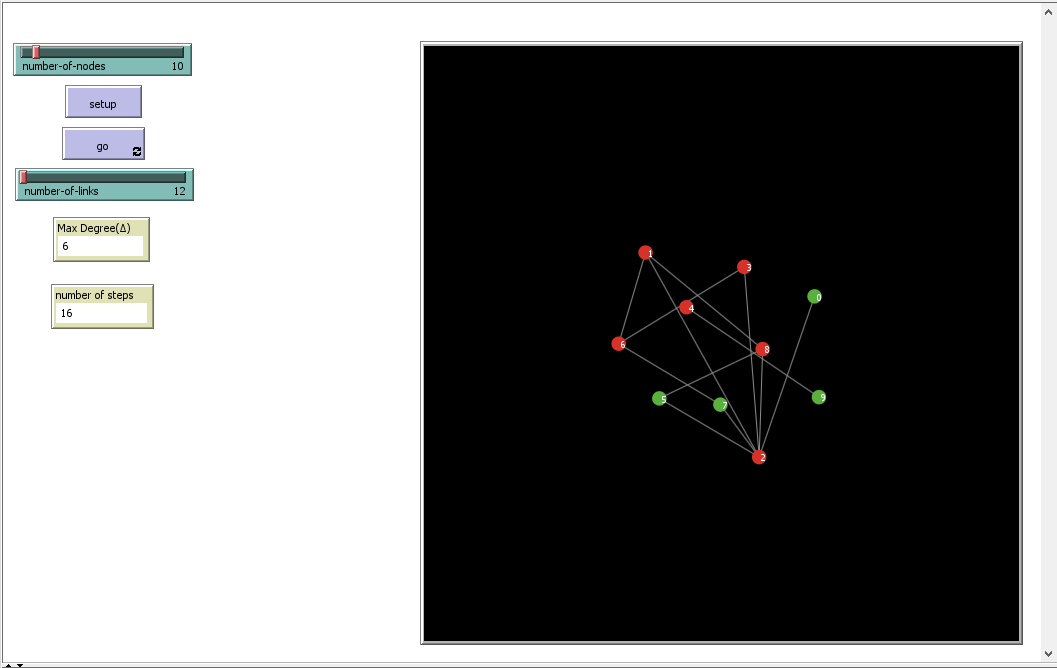
\includegraphics[scale=0.35]{alg1_baselinks.png} }}\\
		\quad
		\subfloat[\centering \en 3n links(n=10)]{{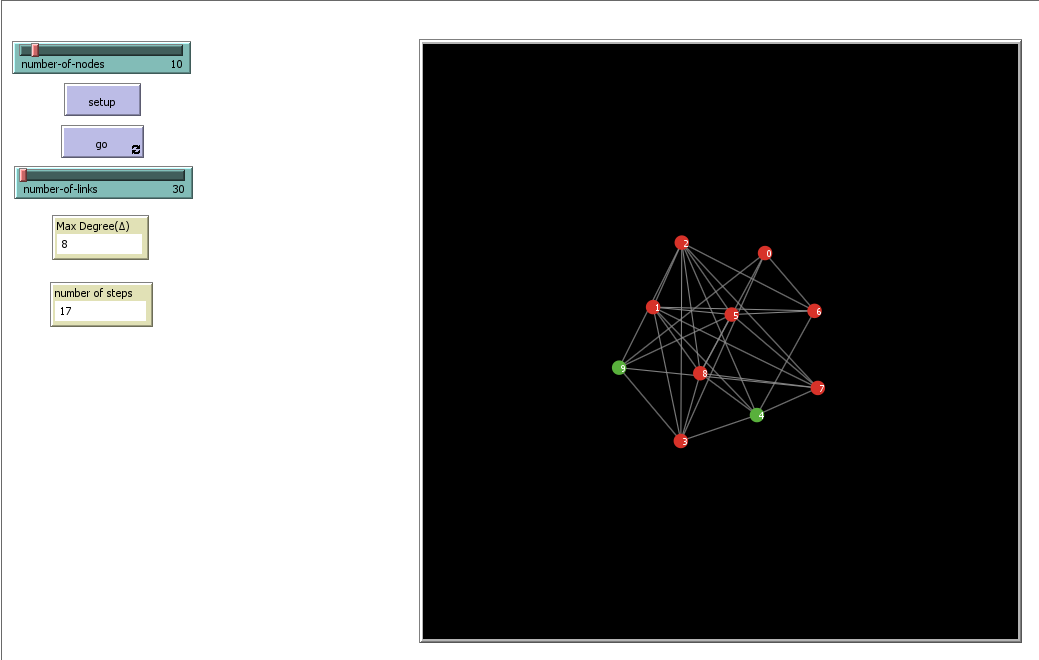
\includegraphics[scale=0.35]{alg1_3n_links.png} }}\\
		\quad
		\subfloat[\centering \en 7n links(n=24)]{{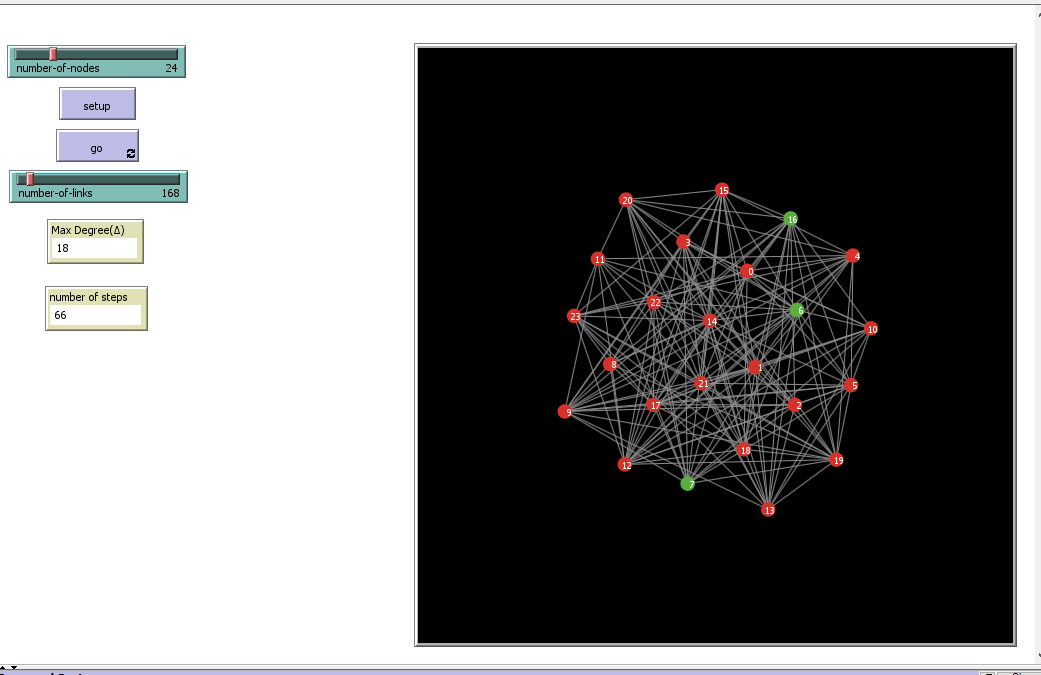
\includegraphics[scale=0.35]{alg1_7n_links(24).png} }}
		\quad
		\subfloat[\centering \en 15n links(n=44)]{{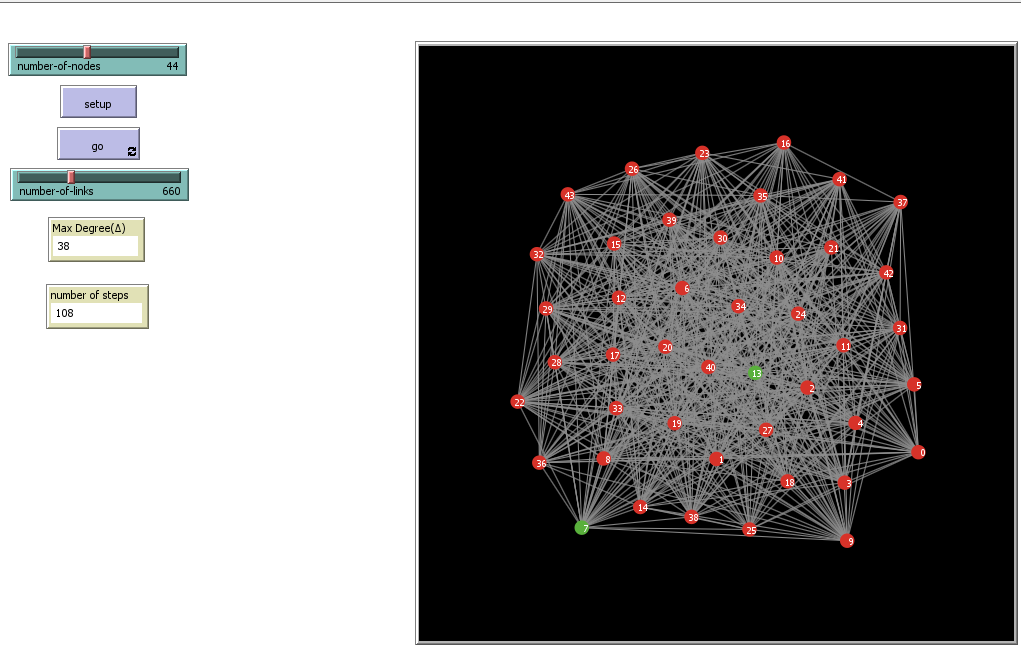
\includegraphics[scale=0.33]{alg1_15n_links(44).png} }}
	\end{figure}		
				
	\begin{figure}[htbp!]
		\center{ \textbf{Αλγόριθμος 2({\en Luby’s MIS Distributed Algorithm}),σελ 17(διαφάνειες)} }
		\centering
		\subfloat[\centering \en Random Example]{{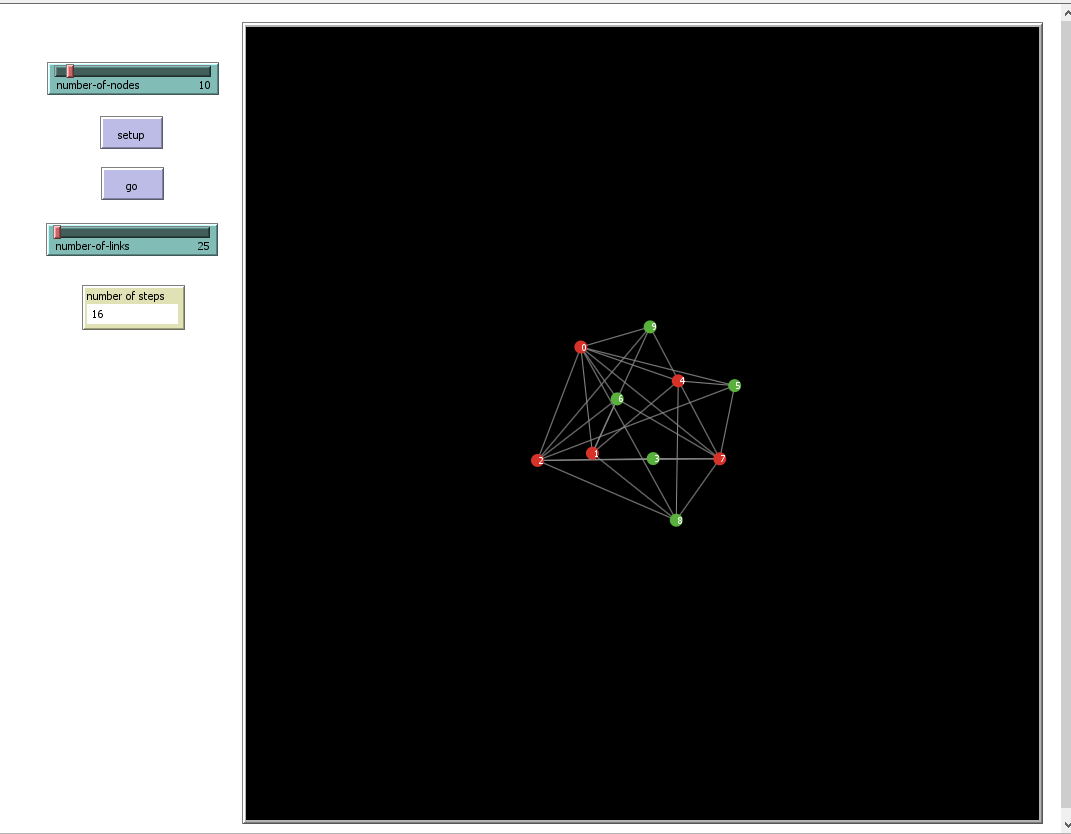
\includegraphics[scale=0.35]{alg2_base_randomlinks.png} }}\\
		\qquad
		\subfloat[\centering \en 3n links(n=10)]{{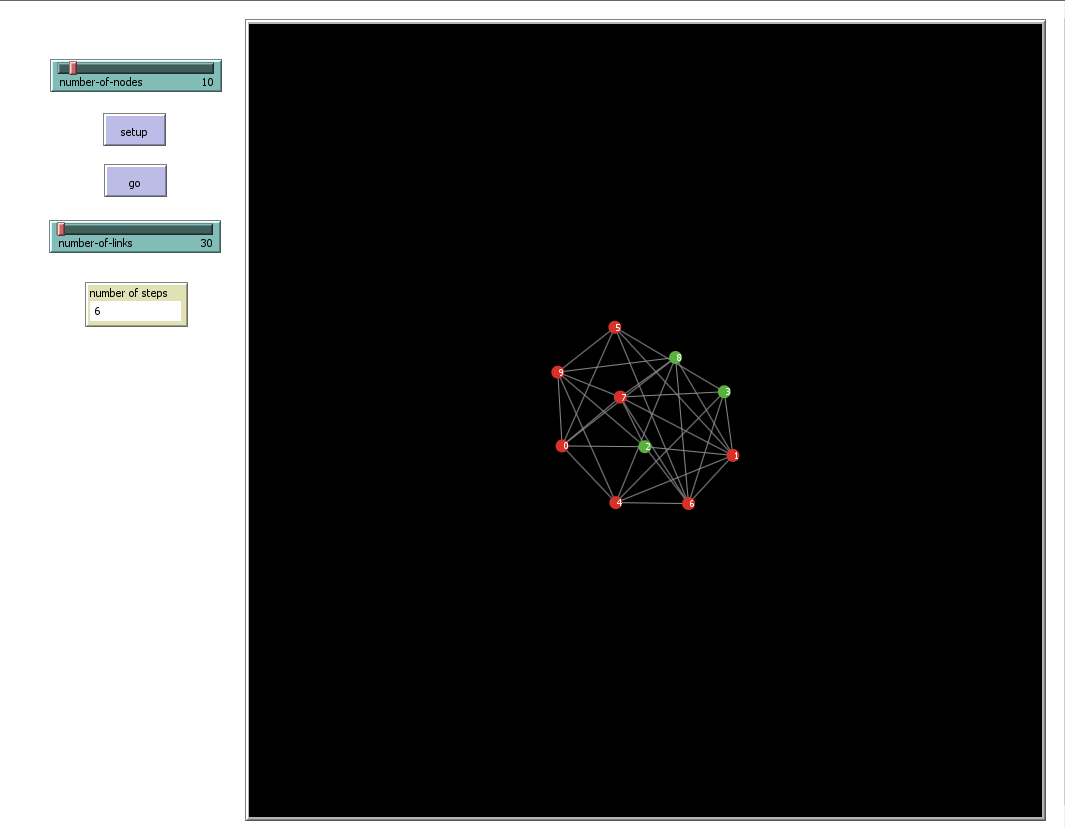
\includegraphics[scale=0.35]{alg2_3n_links.png} }}\\
		\qquad
		\subfloat[\centering \en 7n links(n=35)]{{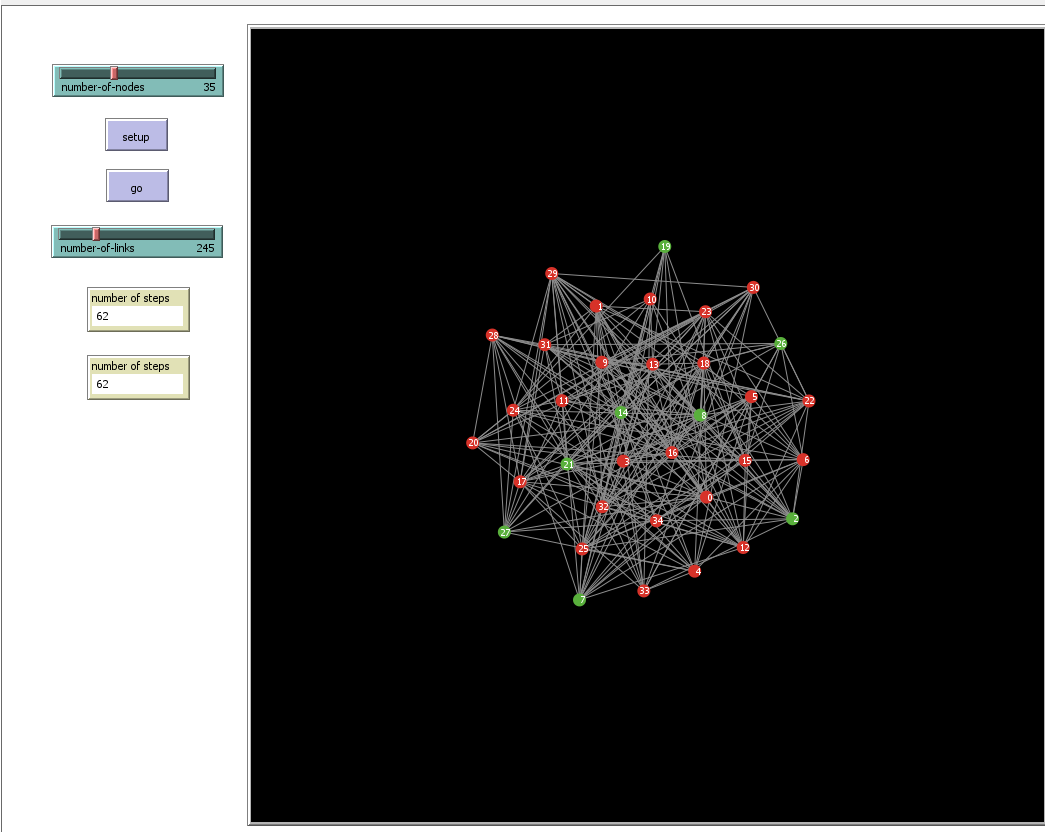
\includegraphics[scale=0.35]{alg2_7n_links(35).png} }}\\
		
		
	\end{figure}		
	
	\newpage
	\begin{figure}[htbp!]
		\centering
	\subfloat[\centering \en 15n links(n=35)]{{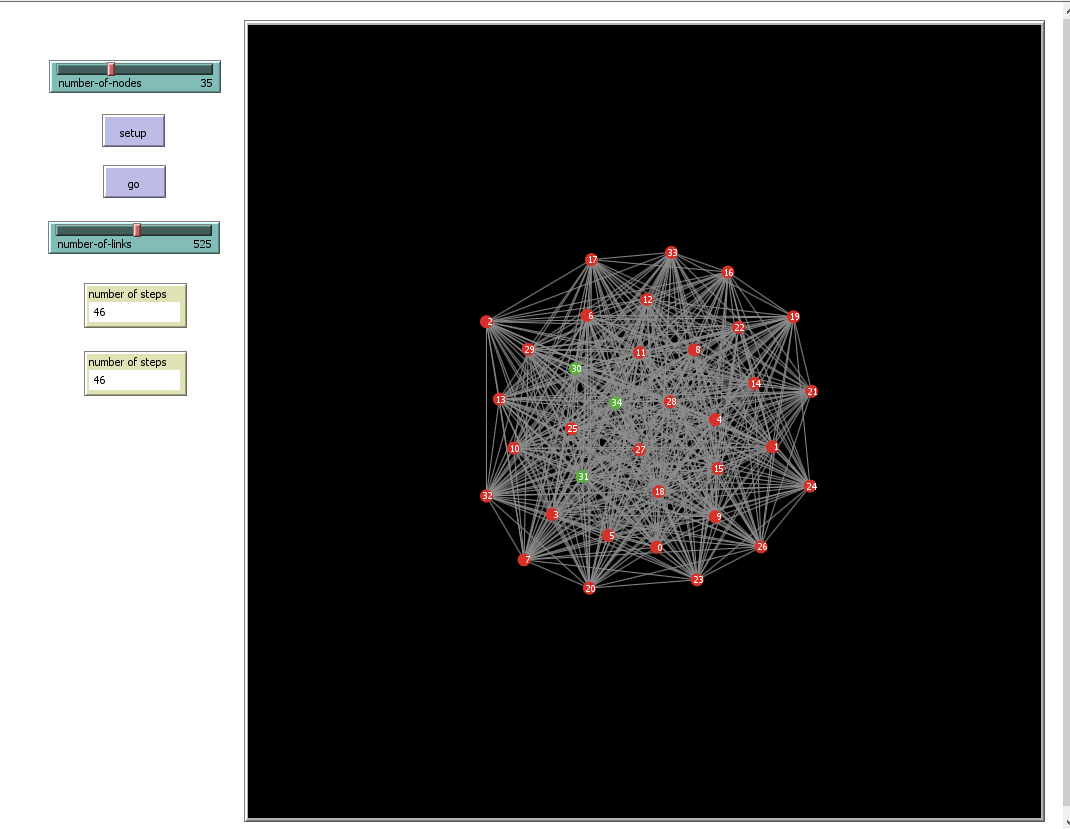
\includegraphics[scale=0.33]{alg2_15n_links(35).png} }}	
    \end{figure}
		
				
			
		\end{document}